\documentclass[11pt]{article}
\usepackage{graphicx}
\DeclareGraphicsExtensions{.eps,.ps,.jpg,.bmp,.png}
\begin{document}

\title{Support Vector Machine(SGD-based)}
\author{Zhiliang Tian}
\date{2016.05.22}
\maketitle
\section{Introduction}
\subsection{What is Support Vector Machine}
Support Vector Machine(SVM), is a two-categories classifier. The thought of original SVM is two norm:
\begin{itemize}
\item Classifing correctly on all observed samples. It means training data accuracy is $100\%$. 
\item Making the distance between different categories as much as they can. Actually, it required making the minimum of distance between different categories as big as they can. The minimum distance is the distance between samples on each categories' boundary.
\end{itemize}
As follow:
\begin{figure}[h!]
    \centering
    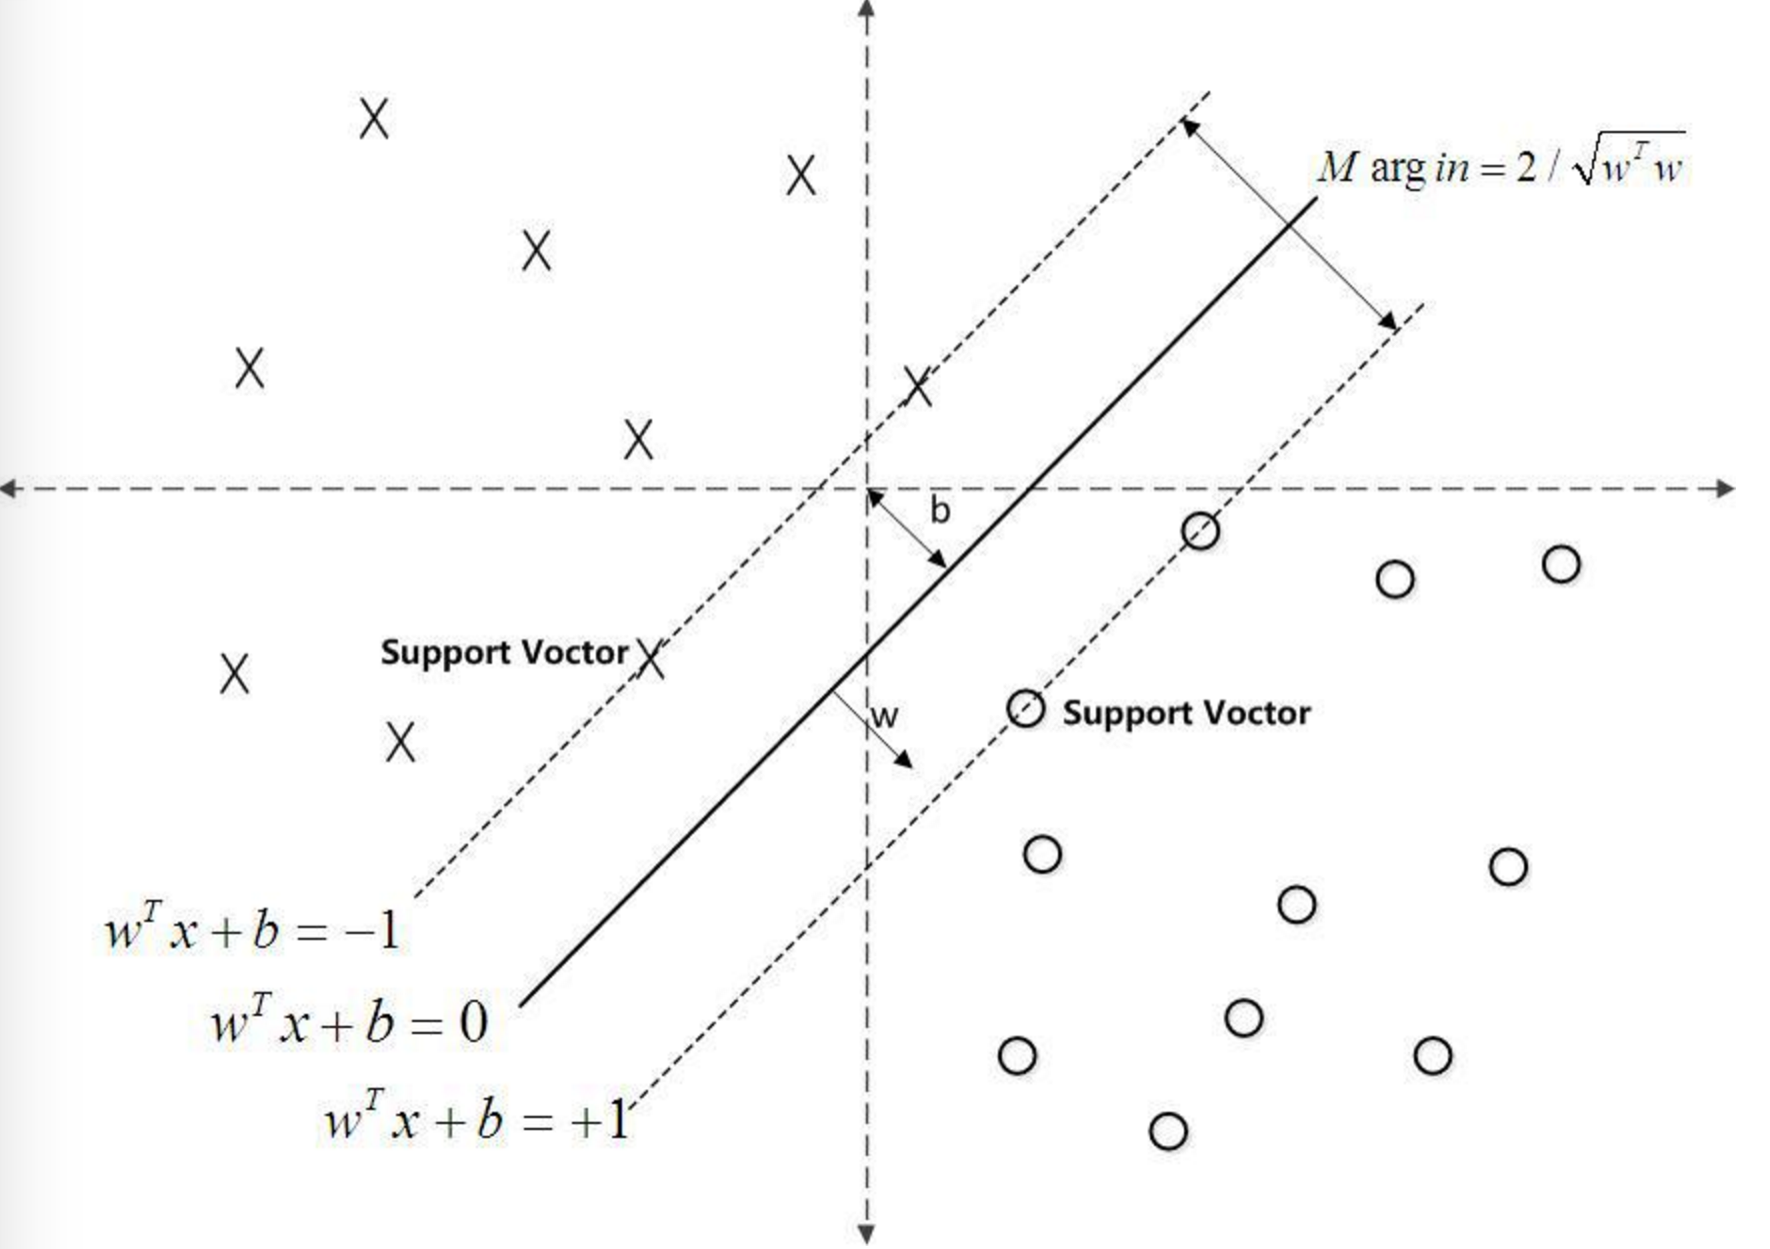
\includegraphics[width=7cm]{f1.png}
    \caption{Svm}
    \label{fig-sample}
\end{figure}

The solid line stands for separating hyperplane(called decision boundary), two dotted lines stand for categories' boundary. The minimum of distance between categories is the gap between dotted lines, called "margin". The sample on categories' boundary decide the margin, called Support Vector. 

\subsection{slack variable and non-linear}
The original SVM can only deal with linearly separable data. If data has some noise(linearly non-separable), we need add slack variable. If data is non-linearly, we need use kernel trick, map data to high-dimension space, then do linear classification there.

\section{classify formula and margin}
\subsection{classify}
This is the formula for classify. given a input feature $\textbf{x}$, f(\textbf{x}) is the output of classifier.
\begin{equation}
\begin{array}{lr}
f(\textbf{x}) = sign(W * \textbf{x} + b) \\
sign(t) =
\left\{
\begin{array}{lr}
1 &              t \geq   0 \\
-1 & t <0 
\end{array}
\right.
\end{array}
\end{equation}
$\textbf{x}$ is a input feature, a vector with $D$ dimension.  $W$ is weight parameter, connecting input feature with output score. $b$ is bias.
On data corpus, the output of each sample $x_i$ is as follow:
\begin{equation}
f(x_i) = sign( \sum_{j=0}^{D}W_j * x_{ij} + b)
\end{equation}
The first norm of SVM require:
\begin{equation}
\begin{array}{lr}
  \forall i  & f(x_i) * y_i > 0
  \end{array}
\end{equation}
$y_i$ is the label of $x_i$.

\subsection{margin}
The second norm of SVM is maximizing the minimum of distance. We use functional margin and geometric margin to evaluate it.
\subsubsection{functional margin}
For all sample $(x_i,y_i)$ in tranning data, ${\gamma}'$ is the functional margin of classifier.
\begin{equation}
\begin{array}{lr}
{\gamma_i}'  = y_i * (\sum_{j=0}^{D}W_j * x_{ij} + b) \\
{\gamma}' = min({\gamma_i}')
\end{array}
\end{equation}

\subsubsection{geometric margin}
For all sample $(x_i,y_i)$ in tranning data, $\gamma$ is the geometric margin of classifier.
\begin{equation}
\begin{array}{lr}
\gamma_i = y_i * f(x_i) = y_i * \frac{(\sum_{j=0}^{D}W_j * x_{ij} + b)}{||W||} \\
\gamma = min(\gamma_i)
\end{array}
\end{equation}

We can see geometric margin is the "normalized version" of functional margin.
\begin{equation}
\gamma = \frac{{\gamma}'}{||W||}
\end{equation}
SVM processing is to ensure classifying correctly on all samples, at the same time to maximize the geometric margin.

\subsection{goal of optimising}
The goal of optimising:
\begin{equation}
\begin{array}{lr}
max  \gamma  \\
s.t.   \forall i & y_i * f(x_i) = y_i * \frac{(\sum_{j=0}^{D}W_j * x_{ij} + b)}{||W||} \geq  \gamma
\end{array}
\end{equation}

\begin{equation}
\begin{array}{lr}
max  \frac{{\gamma}'}{||W||}  \\
s.t.   \forall i & y_i * f(x_i) = y_i * \frac{(\sum_{j=0}^{D}W_j * x_{ij} + b)}{||W||} \geq  {\gamma}'
\end{array}
\end{equation}

Notice that, maximizing $\frac{1}{||W||}$ is totally equal to minimizing $\frac{1}{2} ||W||^2$ (????), so

\begin{equation}
\begin{array}{ll}
max  \frac{1}{2} ||W||^2  \\
s.t.   \forall i & y_i * f(x_i) = y_i * \frac{(\sum_{j=0}^{D}W_j * x_{ij} + b)}{||W||} - 1 \geq  0
\end{array}
\end{equation}

Equation 9 is the final goal of optimising, a convex quadiatic programming.

\section{SGD-based optimising ---- Pegasos}
\subsection{introduction}
Stochastic gradient descent(SGD) ask for a specific loss function. Given a sample, this loss function tell us how to optimize, where should parameter go. Under this loss function, we can approach to final solution sample by sample, using gradient descent. We should balance two norms of SVM.
\subsection{hinge loss and square loss}
\subsubsection{hinge loss}
\begin{equation}
l_h =
\left\{
\begin{array}{lr}
0 &         y_i * f(x_i) - 1 \geq  0      \\
1 - y_i * f(x_i) & y_i * f(x_i) - 1 < 0
\end{array}
\right.
\end{equation}
\begin{equation}
l_h = max(0, 1 - y_i * f(x_i))
\end{equation}
Hinge loss punishes the sample not obey the first norm(the restrict condition in Equation 9)

\subsubsection{square loss}
\begin{equation}
l_s = \frac{1}{2} ||W||^2
\end{equation}
Square loss punishes the L2-norm. It maximizing Equation 9.

\subsubsection{loss}
\begin{equation}
l = \lambda l_s + l_h
\end{equation}
Final loss is the combine of $l_h$ and $l_h$. Pegasos algorithm is similar to it.

\subsection{Pegasos algorithm}
\subsubsection{introduction}
Pegasos algorithm is proposed in 2007, it is a SGD-based optimization of SVM. It seems like a mini-batch gradient descent.
\subsubsection{original definition}
We assume that t is the iterations of minibatch. For $t$-th mini-batch, $A_t$ is the samples set in this batch, $A_t$ contains $k$ samples ($|A_t| = k$).  
\begin{equation}
Loss = \frac{\lambda}{2} ||W||^2 + \frac{1}{k} \sum_{( \textbf x_i,y_i) \in A_t} y_i * f(\textbf x_i)
\end{equation}

\subsubsection{gradient}
At $t$-th iteration:
\begin{equation}
\frac{\alpha(Loss)}{\alpha(W_t)} = \frac{\lambda}{2} * \frac{\alpha( ||W_t||^2)}{\alpha(W_t)} + \frac{1}{k} * \frac{\alpha(\sum_{(x_i,y_i) \in A_t} y_i * f(x_i)}{\alpha(W_t)}
\end{equation}
\begin{equation}
\frac{\alpha(Loss)}{\alpha(W_t)} = \lambda * W_t - \frac{1}{k} * \sum_{(\textbf x_i,y_i)\in A^+_t} y_i * \textbf x_i
\end{equation}

$A^+_t$ is a sample set whose hinge loss is non-zero in $A_t$. We set learning rate $\eta_t = \frac{1}{\lambda * t}$ (why???). 
\begin{equation}
{W}'_{t+1} = W_t - \eta_t \frac{\alpha(Loss)}{\alpha(W_t)} 
\end{equation}
\begin{equation}
{W}'_{t+1} = (1 - \eta_t \lambda) W_t + \frac{\eta_t}{k} \sum_{(\textbf x_i,y_i)\in A^+_t} y_i * \textbf x_i
\end{equation}
${W}'_{t+1}$ is a non-normalization W at $t+1$ iteration.

\subsubsection{normalization}
Then we normalize ${W}'_{t+1}$ (why???). 
We must limit $||W|| \leq 1 / \sqrt{\lambda}$. So, 
\begin{equation}
W_{t+1} = min(1, \frac{1}{\sqrt{\lambda} * ||{W}'_{t+1}|| }) {W}'_{t+1}
\end{equation}
Equation 18 and 19 is a complete mini-batch processing on Pagasos algorithm.

\section{reference and appendix}
\begin{itemize}
\item Original Pegasos. Pegasos: Primal Estimated sub-GrAdient SOlver for SVM
\item Open source. https://github.com/liuhongjiang/blog\_code/blob/master/pegasos
\item My code. https://github.com/tianzhiliang/svm
\end{itemize}

\end{document}

